\section{Fault Injection Simulation for Security Assessment}

\begin{frame}{Fault Injection Simulation for Security Assessment (FISSA)}
    \begin{block}{Presentation}
        \begin{itemize}
            \item Open-Source tool~\cite{fissa}.
            \item Allows the circuit designer to analyse throughout the design cycle the sensibility against FIA.
            \item Integrated around an HDL Simulator (Questasim).
            \item The generated results can help to find vulnerabilities during the design phase.
            \item FISSA enables the principles of Security by Design.
            % \item End-of-simulation statuses are defined by the designer to categorise the simulation.
            \item Presented at DSD 2024~\cite{PLG-24-dsd}.
        \end{itemize}
    \end{block}
\end{frame}

\begin{frame}{FISSA — Software Architecture}
    \begin{figure}
        \centering
        \includegraphics[width=.9\textwidth, page=2]{src/3_fissa/img/fissa/archi_fissa.pdf}
        \caption{FISSA Software Architecture}
        \label{fig:archiSoft}
    \end{figure}
\end{frame}

\begin{frame}{FISSA — Supported Fault Models}
    \begin{table}
        \centering
        \small
        \caption{Supported Fault Model}
        \label{table:supp_fault}
        \setlength{\tabcolsep}{3pt}
        \begin{tabular}{@{}rccc@{}}
            \toprule
            Fault model                                                        & \begin{tabular}[c]{@{}c@{}}Number of\\ target(s)\end{tabular} & \begin{tabular}[c]{@{}c@{}}Number of\\ cycles\end{tabular} & Target size \\
            \midrule
            Set to 0                                                           & 1                                                          & 1                                                          & all         \\
            Set to 1                                                           & 1                                                          & 1                                                          & all         \\
            Single bit-flip in one target at a given clock cycle               & 1                                                          & 1                                                          & all         \\
            Single bit-flip in two targets at a given clock cycle              & 2                                                          & 1                                                          & all         \\
            Single bit-flip in two targets at two different clock cycles       & 2                                                          & 2                                                          & all         \\
            Exhaustive multi-bits faults in one target at a given clock cycle  & 1                                                          & 1                                                          & [1;10] bits \\
            Exhaustive multi-bits faults in two targets at a given clock cycle & 2                                                          & 1                                                          & [1;10] bits \\
            \bottomrule
        \end{tabular}
    \end{table}

    
    \begin{columns}
        \begin{column}{.3\linewidth}
            \hfill
        \end{column}
        \begin{column}{.6\linewidth}
            \begin{itemize}
                \setbeamertemplate{itemize items}[triangle]
                \justifying
            \item All these fault models are used in this work.
        \end{itemize}
        \end{column}
        \begin{column}{.1\linewidth}
            \hfill
        \end{column}
    \end{columns}
\end{frame}